\item \textbf{Wave Equation[1D]}
    \[ y = f\left(\textit{position of particle}, \textit{time}\right) \]
    \begin{center}
        \begin{tikzpicture}
            \def\dl{0.5}
            \def\X{2*pi}
            \def\LT{1}
            \def\F{sin(deg(\x))}
            \begin{scope}[xshift=1cm]
                \tzaxes(0, -1.5)(4.5*pi, 2)
                \tzfn\F[0:4*pi]
                \tzvXpointat{F}{\X}(A)
                \tzcircle(A)(15pt)
                \tzline+[->]($(A)+(0, -15pt)$)(0, -3)
            \end{scope}
            \begin{scope}[yshift=-8cm, scale=2, xshift=-2.5cm]
                \tzfn"arc"\F[\X-2*\LT:\X+2*\LT]
                \tzfn[line width=1mm]\F[\X - 0.5*\dl:\X + 0.5*\dl]
                \tzvXpointat{F}{\X}(A)
                %\tzcircle(A)(35pt) 
                \tzvXpointat*{F}{\X - 0.5*\dl}(START)
                \tzvXpointat*{F}{\X + 0.5*\dl}(END)
                \tztangent[->]"TL"{arc}(START)[\X-0.5*\dl:\X-\LT]{$T_1$}[b]
                \tztangent[->]"TR"{arc}(END)[\X+0.5*\dl:\X+\LT]{$T_2$}
                \tzline+[dashed](START)(-1, 0)
                \tzline+[dashed](START)(1, 0)
                \tzline+[dashed](END)(1, 0)
                \tzvXpointat{TR}{\X+1}(TRP)
                \tzanglemark($(START)+(1, 0)$)(START)(END){$\theta$}(8pt)
                \tzanglemark($(END)+(1, 0)$)(END)(TRP){$\theta + \d{\theta}$}[r](8pt)
                \tzline+[->](END)(1.5, 0){$T_2\cos(\theta+\d{\theta})$}[r]
                \tzline+[->](END)(0, 1.5){$T_2\sin(\theta+\d{\theta})$}[a]
                \tzline+[->](START)(0, -1.5){$T_1\sin(\theta)$}[b]
                \tzline+[->](START)(-1.5, 0){$T_1\cos(\theta)$}[l]
            \end{scope}
        \end{tikzpicture}
    \end{center}
    \begin{align*}
        \intertext{Above diagram shows a small segment of the string.}
        \intertext{Force along the horizontal direction will get balanced out, cause the string won't accelerate along horizontal.}
        T_2\cos(\theta+\d{\theta}) - T_1\cos(\theta) &= 0\\
        \Aboxed{T_1 &= T_2} \tag{1}\\
        \intertext{Force along the vertical direction won't be balanced out, cause the string will accelerate along vertical.}
        T_2\sin(\theta+\d{\theta}) - T_1\sin(\theta) &= m a_y\\
        \intertext{As string will perform small oscillations, $\theta$ will be small.}
        T_2\left(\theta + \d{\theta}\right) - T_1\theta &= m a_y\\
        \intertext{Also, the mass of this small segment will $\d{m}$,}
        T_2\left(\theta + \d{\theta}\right) - T_1\theta &= \d{m} a_y\\
        \intertext{Because of small oscillations length of this segment will be $\d{x}$ so, $\d{m} = \upmu \d{x}$, $T_1=T_2=T$}
        T_2\left(\theta + \d{\theta}\right) - T_1\theta &= \upmu \d{x} a_y\\
        T\d{\theta} &= \upmu \d{x} a_y\\
        \Aboxed{\dfrac{\d{\theta}}{\d{x}} &= \dfrac{\upmu}{T} a_y } \tag{2}\\
        \intertext{Also we have,}
        \dfrac{\d{y}}{\d{x}} &= \tan(\theta)\\
        \dfrac{\d^2{y}}{\d{x^2}} &= \sec^2\theta\dfrac{\d{\theta}}{\d{x}}\\
        \Aboxed{\dfrac{\d{\theta}}{\d{x}} &= \dfrac{\d^2{y}}{\d{x^2}}} \tag{3}\\
        \intertext{Combining both equations,}
        \dfrac{\d^2{y}}{\d{x^2}} &= \dfrac{\upmu}{T} a_y\\
        \intertext{As we know, $a_y = \dfrac{\partial^2{y}}{\partial{t^2}}$ and $\dfrac{\d^2{y}}{\d{x^2}}=\dfrac{\partial^2{y}}{\partial{x^2}}$}
        \Aboxed{\dfrac{\partial^2{y}}{\partial{x^2}} &= \dfrac{\upmu}{T} \dfrac{\partial^2{y}}{\partial{t^2}}} \tag{\textit{Wave Equation}}
    \end{align*}

    \item \textbf{Solution of above differential equation}
    \begin{align*}
        \intertext{Solving the above differential equation is beyond the scope of this article. But the solution is,}
        y(x, t) &= f\left(k x \pm \omega t\right)\\
        \intertext{Any function of the form $f\left(k x \pm \omega t\right)$ will satisfy the wave equation.}
        \intertext{Let's see what we get if we differentiate $y(x, t)$ with respect to $t$ and $x$.}
        \dfrac{\partial{y}}{\partial{t}} &= \pm \omega f'\left(k x \pm \omega t\right)\\
        \dfrac{\partial^2{y}}{\partial{t^2}} &= \omega^2 f''\left(k x \pm \omega t\right)\tag{1}\\
        \intertext{Similarly,}
        \dfrac{\partial{y}}{\partial{x}} &= k f'\left(k x \pm \omega t\right)\\
        \dfrac{\partial^2{y}}{\partial{x^2}} &= k^2 f''\left(k x \pm \omega t\right)\tag{2}\\
        \intertext{Substituting (1) and (2) in the wave equation,}
        k^2 f''\left(k x \pm \omega t\right) &= \dfrac{\upmu}{T} \omega^2 f''\left(k x \pm \omega t\right)\\
        \omega^2 &= \dfrac{\upmu}{T} k^2\\
        \Aboxed{\sqrt{\dfrac{T}{\upmu}} &= \dfrac{\omega}{k}} \\
    \end{align*}
    \pagebreak

    \item \textbf{Speed of wave}
    \begin{center}
        \begin{tikzpicture}
            \foreach \I [evaluate={\i=-\I*1.5}] in {0, 1,..., 5}{
                \tzcoor*(0, \i)(A)
                \tzcoor(10, \i)(B){$t=t_\I$}[r]
                \ifthenelse{\I=0}{\tzline+[<->]($(A)+(0, -0.5)$)(0, 1)}{}
                \tzline+(A)(-\i, 0)
                \tzfn<-\i, \i>{0.5*sin(deg(2*\x))}[0:0.5*pi]
                \tzline+(-\i + 0.5* pi, \i)(8+\i, 0)
                \tzline+[->]<0, 0.5>(-\i+0.25*pi, \i)(1, 0){$v$}[r]
            }
        \end{tikzpicture}
        \begin{tikzpicture}
            \def\dl{1}
            \def\X{0.5*pi}
            \def\LT{1.5}
            \def\F{sin(deg(\x))}
            \begin{scope}
                \tzfn"arc"\F[\X-2*\LT:\X+2*\LT]
                \tzfn[line width=1mm]\F[\X - 0.5*\dl:\X + 0.5*\dl]
                \tzvXpointat{F}{\X}(A)
                %\tzcircle(A)(35pt) 
                \tzvXpointat*{F}{\X - 0.5*\dl}(START)
                \tzvXpointat*{F}{\X + 0.5*\dl}(END)
                \tztangent[->]"TL"{arc}(START)[\X-0.5*\dl:\X-\LT]{$T_1$}[l]
                \tztangent[->]"TR"{arc}(END)[\X+0.5*\dl:\X+\LT]{$T_2$}[r]
                \tzvXpointat{TR}{\X+1}(TRP)
                \tzvXpointat{TL}{\X-1}(TLP)
                \tzanglemark($(START)+(-1, 0)$)(START)(TLP){$\theta$}(12pt)
                \tzanglemark'($(END)+(1, 0)$)(END)(TRP){$\theta$}[r](12pt)
                \tzline+[->](END)(1.5, 0){$T_2\cos(\theta)$}[r]
                %\tzline+[->](END)(0, -1.5){$T_2\sin(\theta+\d{\theta})$}[a]
                %\tzline+[->](START)(0, -1.5){$T_1\sin(\theta)$}[b]
                \tzline+[->](START)(-1.5, 0){$T_1\cos(\theta)$}[l]
                \tzline"RL"($(START)!0.01!(TLP)$)($(START)!1.2cm!90:($(START)!0.01!(TLP)$)$)
                \tzline"RR"($(END)!0.01!(TRP)$)($(END)!-1.2cm!90:($(END)!0.01!(TRP)$)$)
                \tzXpoint*{RL}{RR}(O)
                \tzanglemark(END)(O)(START){$2\theta$}(12pt)
            \end{scope}
            \begin{scope}[xshift=8cm]
                \tzfn"arc"\F[\X-2*\LT:\X+2*\LT]
                \tzfn[line width=1mm]\F[\X - 0.5*\dl:\X + 0.5*\dl]
                \tzvXpointat{F}{\X}(A)
                %\tzcircle(A)(35pt) 
                \tzvXpointat*{F}{\X - 0.5*\dl}(START)
                \tzvXpointat*{F}{\X + 0.5*\dl}(END)
                \tztangent[->]"TL"{arc}(START)[\X-0.5*\dl:\X-\LT]{$T_1$}[l]
                \tztangent[->]"TR"{arc}(END)[\X+0.5*\dl:\X+\LT]{$T_2$}[r]
                \tzline+[->](A)(1.5, 0){$v$}[r]
                \tzline+[->](A)(0, -1.5){$a_r$}[b]
            \end{scope}
        \end{tikzpicture}
    \end{center}
    \begin{align*}
        \intertext{As we can see in the above diagram, the wave is moving with a velocity $v$(actually the string is moving but in the case of mechanical wave it acts as a carrier of energy and momentum, hence we can assume speed of the wave will be same as the string) and the segment of string will have a radial acceleration($a_r$)}\\
        F_x &= 0\\
        F_y &= m a_r\\
        2T\sin\theta &= \dfrac{mv^2}{r}\\
        \intertext{As $\theta$ is small, $\sin\theta \approx \theta$}
        2T\theta &= \dfrac{\upmu \cdot r \cdot 2\theta v^2}{r}\\
        v^2 &= \dfrac{T}{\upmu}\\
        \Aboxed{v &= \sqrt{\dfrac{T}{\upmu}}}\tag{wave velocity}\\
        \intertext{Now, we can summarize the above discussion in a single equation,}
        \Aboxed{\dfrac{\partial^2{y}}{\partial{t^2}} = v^2\dfrac{\partial^2{y}}{\partial{x^2}}, \quad v = \sqrt{\dfrac{T}{\upmu}}, \quad v &=\dfrac{\omega}{k}=\dfrac{\textit{coefficient of time(t)}}{\textit{coefficient of space(x)}}}
    \end{align*}
    \pagebreak

    \item \textbf{Another look at wave velocity}
    \begin{center}
        \begin{tikzpicture}
            \tzaxes(0, -1)(4.5*pi, 2){$x$}{$y$}
            \tzfn"curve"{sin(deg(\x))}[0:4*pi]
            \foreach \x in {0.5*pi, 1.5*pi, 2.5*pi, 3.5*pi}{
                \tzvXpointat*{curve}{\x}(A)
                \tzline+[->](A)(1, 0){$v$}[r]
            }
            % \foreach \I [evaluate={\i=-\I*1.5}] in {0, 1, 2}{
            %     \tzcoor*(0, \i)(A)
            %     \tzcoor(10, \i)(B){$t=t_\I$}[r]
            %     \ifthenelse{\I=0}{\tzline+[<->]($(A)+(0, -0.5)$)(0, 1)}{}
            %     \tzline+(A)(-\i, 0)
            %     \tzfn<-\i, \i>{0.5*sin(deg(2*\x))}[0:0.5*pi]
            %     \tzline+(-\i + 0.5* pi, \i)(8+\i, 0)
            %     \tzline+[->]<0, 0.5>(-\i+0.25*pi, \i)(1, 0){$v$}[r]
            % }
        \end{tikzpicture}
    \end{center}
    \begin{align*}
        y(x, t) &= f\left(k x \pm \omega t + \phi\right)
        \intertext{For simplicity, let's assume a sine wave.}
        \intertext{Every peak is moving with a velocity $v$, this velocity is the velocity of the wave.}
        \intertext{This is the fun part, }
        \intertext{Rate at which peak is moving is $\dfrac{\d{x}}{\d{t}}$,}
        \intertext{To get peak, $kx \pm \omega t + \phi$ must be odd integral multiple of $\dfrac{\pi}{2}$,}
        kx \pm \omega t + \phi &= \left(2n+1\right)\dfrac{\pi}{2}
        \intertext{Differentiating both sides with respect to $t$,}
        k\dfrac{\d{x}}{\d{t}} \pm \omega &= 0\\
        \Aboxed{\dfrac{\d{x}}{\d{t}} &= \mp \dfrac{\omega}{k}}\\
        \intertext{This concludes an important result,}
    \end{align*}
    \vspace*{-60mm}
    \begin{center}
        \begin{tikzpicture}
            \tzaxes(0, -1)(4.5*pi, 1.5){$x$}{$y$}
            \tzfn"curve"{sin(deg(\x))}[0:4*pi]
            \foreach \x in {0.1, 0.2, ..., 4}{
                \tzvXpointat*{curve}{\x*pi}(A)
                \tzline+[->](A)(1, 0)
            }
        \end{tikzpicture}
    \end{center}
    \begin{align*}
        \intertext{Although we assumed only for peaks, but it is true for any point, because all the points are moving in the same fashion.}
        \intertext{For $y(x, t)=f(kx-\omega t + \phi)$, wave will move in the positive direction,}
        \Aboxed{v &= \dfrac{\omega}{k}}\\
        \intertext{For $y(x, t)=f(kx+\omega t + \phi)$, wave will move in the negative direction,}
        \Aboxed{v &= -\dfrac{\omega}{k}}
    \end{align*}
